\documentclass[a4paper,12pt]{report}

\usepackage[T1]{fontenc}
\usepackage[francais]{babel}
\usepackage[a4paper, margin=2cm]{geometry}
\usepackage[utf8]{inputenc}
\usepackage{graphicx}


\begin{document}

Pour assurer une rentabilité à notre projet, il nous faut le penser, le structurer en vue d'une large distribution sous de multiples formes.


\subsection{Choix d'une architecture optimale pour notre projet}

Distribuer notre projet tel quel présenterait à ce stade de nombreux défauts:
- le coeur de notre technologie de reconnaissance vocale est directement accessible à tous.
- une interface unique en ligne de commande constitue un blocage majeur pour la majorité des utilisateurs finaux et empêche une intégration large à des applications tierces.

\bigskip

\textbf{\emph{Étudions l'opportunité d'adopter une architecture client/serveur pour ce projet.}}

\bigskip

Dans ce scénario, divers clients logiciels, potentiellement indépendant de The SpeechApp Company pourraient communiquer par requêtes/réponses (spécifiées par une API) aves les serveurs de The SpeechApp Company. Ces derniers seuls auraient accès au coeur algorithmique du projet, qui resterait ainsi exclusivement entre nos mains. Par leurs requêtes, les clients demanderaient l'analyse automatique de mots, l'ajout de nouveaux mots ainsi que toute autre opération pertinentes relative à l'analyse et la gestion d'une base de données de mots. L'accès à notre API serait monétisable forfaitairement ou à l'utilisation.

\medskip

Les mots enregistrés par les clients seraient conservés dans des bases de données chez The SpeechApp Company. La location de ses bases de données hebergées serait monétisable.
Alors, The SpeechApp Company pourrait prioritairement développer deux applications connectables au serveur : la première, SpeechCreator, permettrait l'enregistrement aisé de nouveaux mots dans les bases de données clients. La seconde, SpeechApp, permettrait, au travers d'une application Web riche, de tester la reconnaissance vocale en ligne.

\medskip

Cette configuration permettrait aussi à une multitudes d'applications tierces d'utiliser notre technologie en ne voyant de l'extérieur qu'une API définissant le format des requêtes et réponses dans la communication entre clients logiciel et serveur.

\medskip

Nous aboutirions alors à l'architecture représentée par le schéma suivant:

\begin{figure}
	\begin{center}
	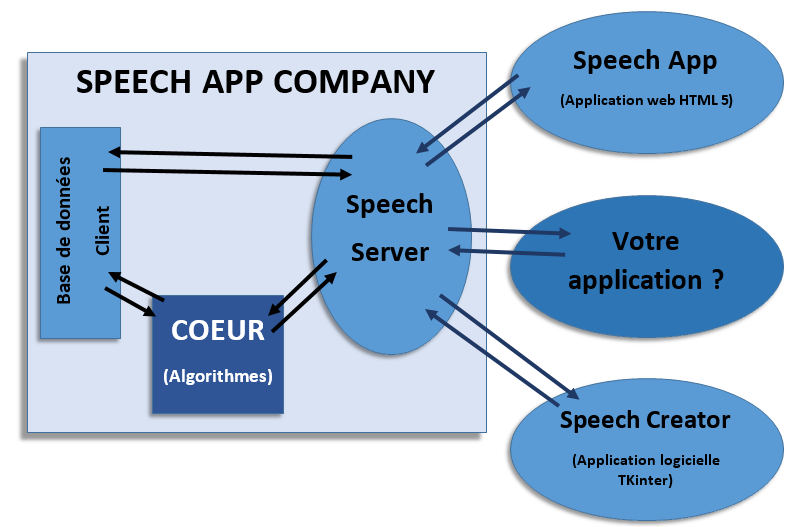
\includegraphics[width=14cm]{pics/architecture.png} 
	\end{center}
	\caption{Architecture proposée pour le projet The SpeechApp Company}
\end{figure}

Plus précisement dans le cadre des échanges entre le SpeechServer
Les requêtes pourraient être traitées de la façon suivante :
Le client (au sens logiciel toujours) envoie au SpeechServer une requête HTTP POST contenant un formulaire avec en particulier son identifiant, son mot de passe, la base de données qu'il veut utiliser, l'action qu'il veut faire effectuer au SpeechServer, et les données d'entrée qui lui sont associées.
La requête analysée par le SpeechServer, les opérations adéquates ayant été réalisées par le coeur algorithmique, le SpeechServer répond au client par une réponse HTTP POST contenant des données au format XML.
Le client peut alors lire et interpreter la réponse donnée par le SpeechServer.

\bigskip

Avec ses spécifications, nous obtiendrions le cycle suivant pour la reconnaissance d'un mot par SpeechApp :

\begin{figure}
	\begin{center}
	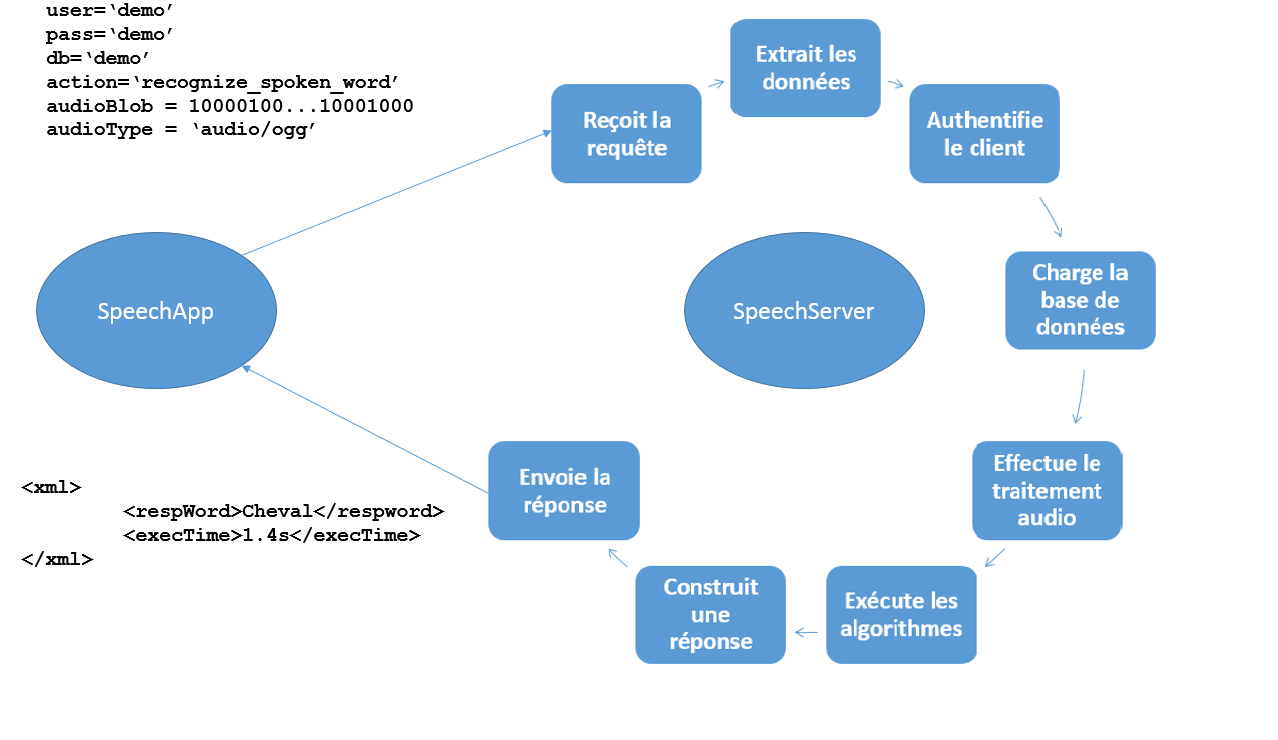
\includegraphics[width=14cm]{pics/vieRequete.png} 
	\end{center}
	\caption{Reconnaissance d'un mot par SpeechApp couplée au SpeechServer}
\end{figure}

\emph{L'architecture client/serveur proposée présenterai pour nous l'avantage de}
\begin{itemize}
	\item{permettre la création d'un écosystème varié d'applications basées sur le coeur algorithmique de The SpeechApp Company via l'API de son SpeechServer, et générant ainsi des revenus}
	\item{conserver le coeur de notre travail entre nos mains et même de nous donner le contrôle sur toute la chaîne}
\end{itemize}

\medskip{}

\emph{L'architecture client/serveur proposée présenterai pour nos clients l'avantage de}
\begin{itemize}
	\item{ne pas se soucier du coeur algorithmique de la reconnaissance vocale, en n'y voyant que l'API de SpeechServer. Cette API peut offrir par ailleurs une grande liberté d'action}
	\item{n'avoir pas ou peu d'investissement initial de développement à effectuer, nos applications propriétaires SpeechApp et SpeechRecorder pouvant être intégrées sous forme de widgets aux applications tierces}
	\item{ne pas avoir a faire de lourds calculs eux-mêmes, ceux-ci étant réalisés par les machines de The SpeechApp Company}
	\item{les cycles de mises à jour seraient en majorité invisibles chez les clients, l'API restant immuables sur des cycles plus long (Long Term Support)}
\end{itemize}

Au vu des nombreux avantages qu'elle présente,
\emph{Nous avons donc opté pour une architecture modulaire client/serveur pour notre projet.}

\subsection{Réalisation du SpeechServer}

Le SpeechServer a été codé en Python. Python a une libraire standard suffisamment riche pour n'avoir a traiter ce problème qu'à un haut niveau (en reception de requêtes selon leurs méthodes). De plus, ce choix facilite les interactions avec le coeur algorithmique : des imports et appels de fonctions depuis le SpeechServer suffisent.

\medskip{}

Finalement, le SpeechServer prend seulement la forme d'un programme python à lancer sur un ordinateur.

\begin{figure}
	\begin{center}
	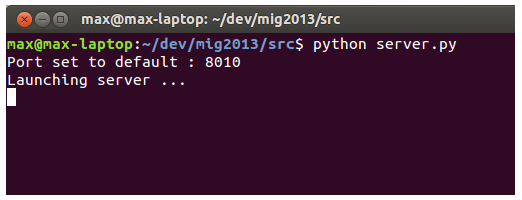
\includegraphics[width=14cm]{pics/server.png} 
	\end{center}
	\caption{Le SpeechServer lancé}
\end{figure}

Il écoute alors les requêtes sur le port 8010 (par défaut) de l'ordinateur. Lorsqu'il en reçoit, il interragit avec le coeur algorithmique et le système de gestion de bases de données mis en place.

\subsection{Système de Gestion de Base de Données (SGBD)}

Le SGBD doit permettre de stocker et gérer les fichiers audio associés aux mots (au moins une dizaine d'enregistrement par mot), les modèles de markov cachés qui leurs sont associés ainsi que les données d'authenfication des applications clientes.

\medskip{}

Le standard actuel de gestion de bases de données est le modèle relationnel basé sur le langage SQL. Néanmoins, dans le cas précis de stockage de fichiers relativement lourds (> 0.1 Mo), la lecture/écriture des données directemnt sur le disque dur s'avère plus performante.

\medskip{}

Nous avons donc fait le choix de stocker nos données sur le disque dur du serveur, en enregistrant les fichiers audio en format brut, et les autres données (modèles de Markov, données d'authentification) comme des objets Python, avec le module pickle de la librairie standard.

\smallskip{}

Un module python db.py a été developpé par nos soins pour gérer efficacement nos fichiers

\bigskip{}

Comme les accès en lecture/écriture à la mémoire RAM sont bien plus rapide que les accès aux disques dur,
\emph{On pourrait obtenir un gain de vitesse significatif pour la reconnaissance vocale en chargeant l'intégralité des données en mémoire RAM au démarrage du SpeechServer}
Néanmoins, la quantité de mémoire RAM nécessaire serait très importante, croissant exponentiellement avec le nombre de mots enregistrés. Les coûts engendrés seraient importants :

\medskip{}

Sur la gamme serveurs de calcul de l'hébergeur OVH,
Le serveur doté de 256 Go de RAM est loué 300 € HT / mois.
Le même serveur (en termes de performance CPU et de disque dur : 4 To) doté de 64 Go de RAM, est loué 80 € HT / mois

\medskip{}

Un système hybride de cache en mémoire RAM pourrait aussi être envisagé, mais nous n'avons pas le temps de le mettre en place en moins de 3 semaines.

\medskip{}

\emph{On conservera un stockage des données intégralement sur disque dur}

\medskip{}
Les spécifications du SpeechServer et de du SGBD ayant été définis, il devient possible de construire des applications se fondant dessus.

\subsection{SpeechApp}

\subsection{SpeechRecorder}

\end{document}





